\chapter{Methodology}\label{chap:methodology}

\section{Dataset}

Our dataset is derived from the publically available Face Research Lab London~\cite{frll} (FRLL) set, comprising 102, $1350 \times 1350$, full coloured images of frontal, ICAO-compliant adult faces. Self-reported age, gender and ethnicity are included. Attractiveness ratings (on a 1--7 scale from ``much less attractiveness than average'' to ``much more attractive than average'') for the faces from 2513 people (ages 17--90) are included as well. The FRLL dataset was selected for its high-fidelity ICAO-compliant images, controlled acquisition conditions, and extensive demographic annotations, which are crucial for analyzing perceptual quality and potential demographic biases in subjective ratings. Each image was encoded using four printer-proof steganographic methods, each applied at nine different intensity levels, $x \mid x = 0.6 + 0.1 \times k, k \in \{0, \hdots, 8\}$, yielding a total of 3,672 distorted images.

The dataset was partitioned into four subsets, as follows:

\begin{itemize}
    \item MOS set (15 identities, 540 images): a core set of demographically diverse subjects, shown in Fig.~\ref{fig:mos_set}, with subjective MOS annotations. It is split into:
    \begin{itemize}
        \item MOS train set (12 identities): used to train the FR fusion model, regressing FR-IQA metrics to human MOS.\@
        \item MOS test set (3 identities): held out from the framework and used only for final evaluation.
    \end{itemize}
    \item Pseudo-MOS set (87 identities, 3,132 images): no subjective scores were collected for these images. Pseudo-MOS are generated for this set using the trained fusion model.
    \item NR train set: includes both the MOS train set and the pseudo-MOS set. It is used to train the NR regressor.
\end{itemize}

\begin{figure}
    \centering
    \begin{subfigure}{0.76\textwidth}
        \centering
        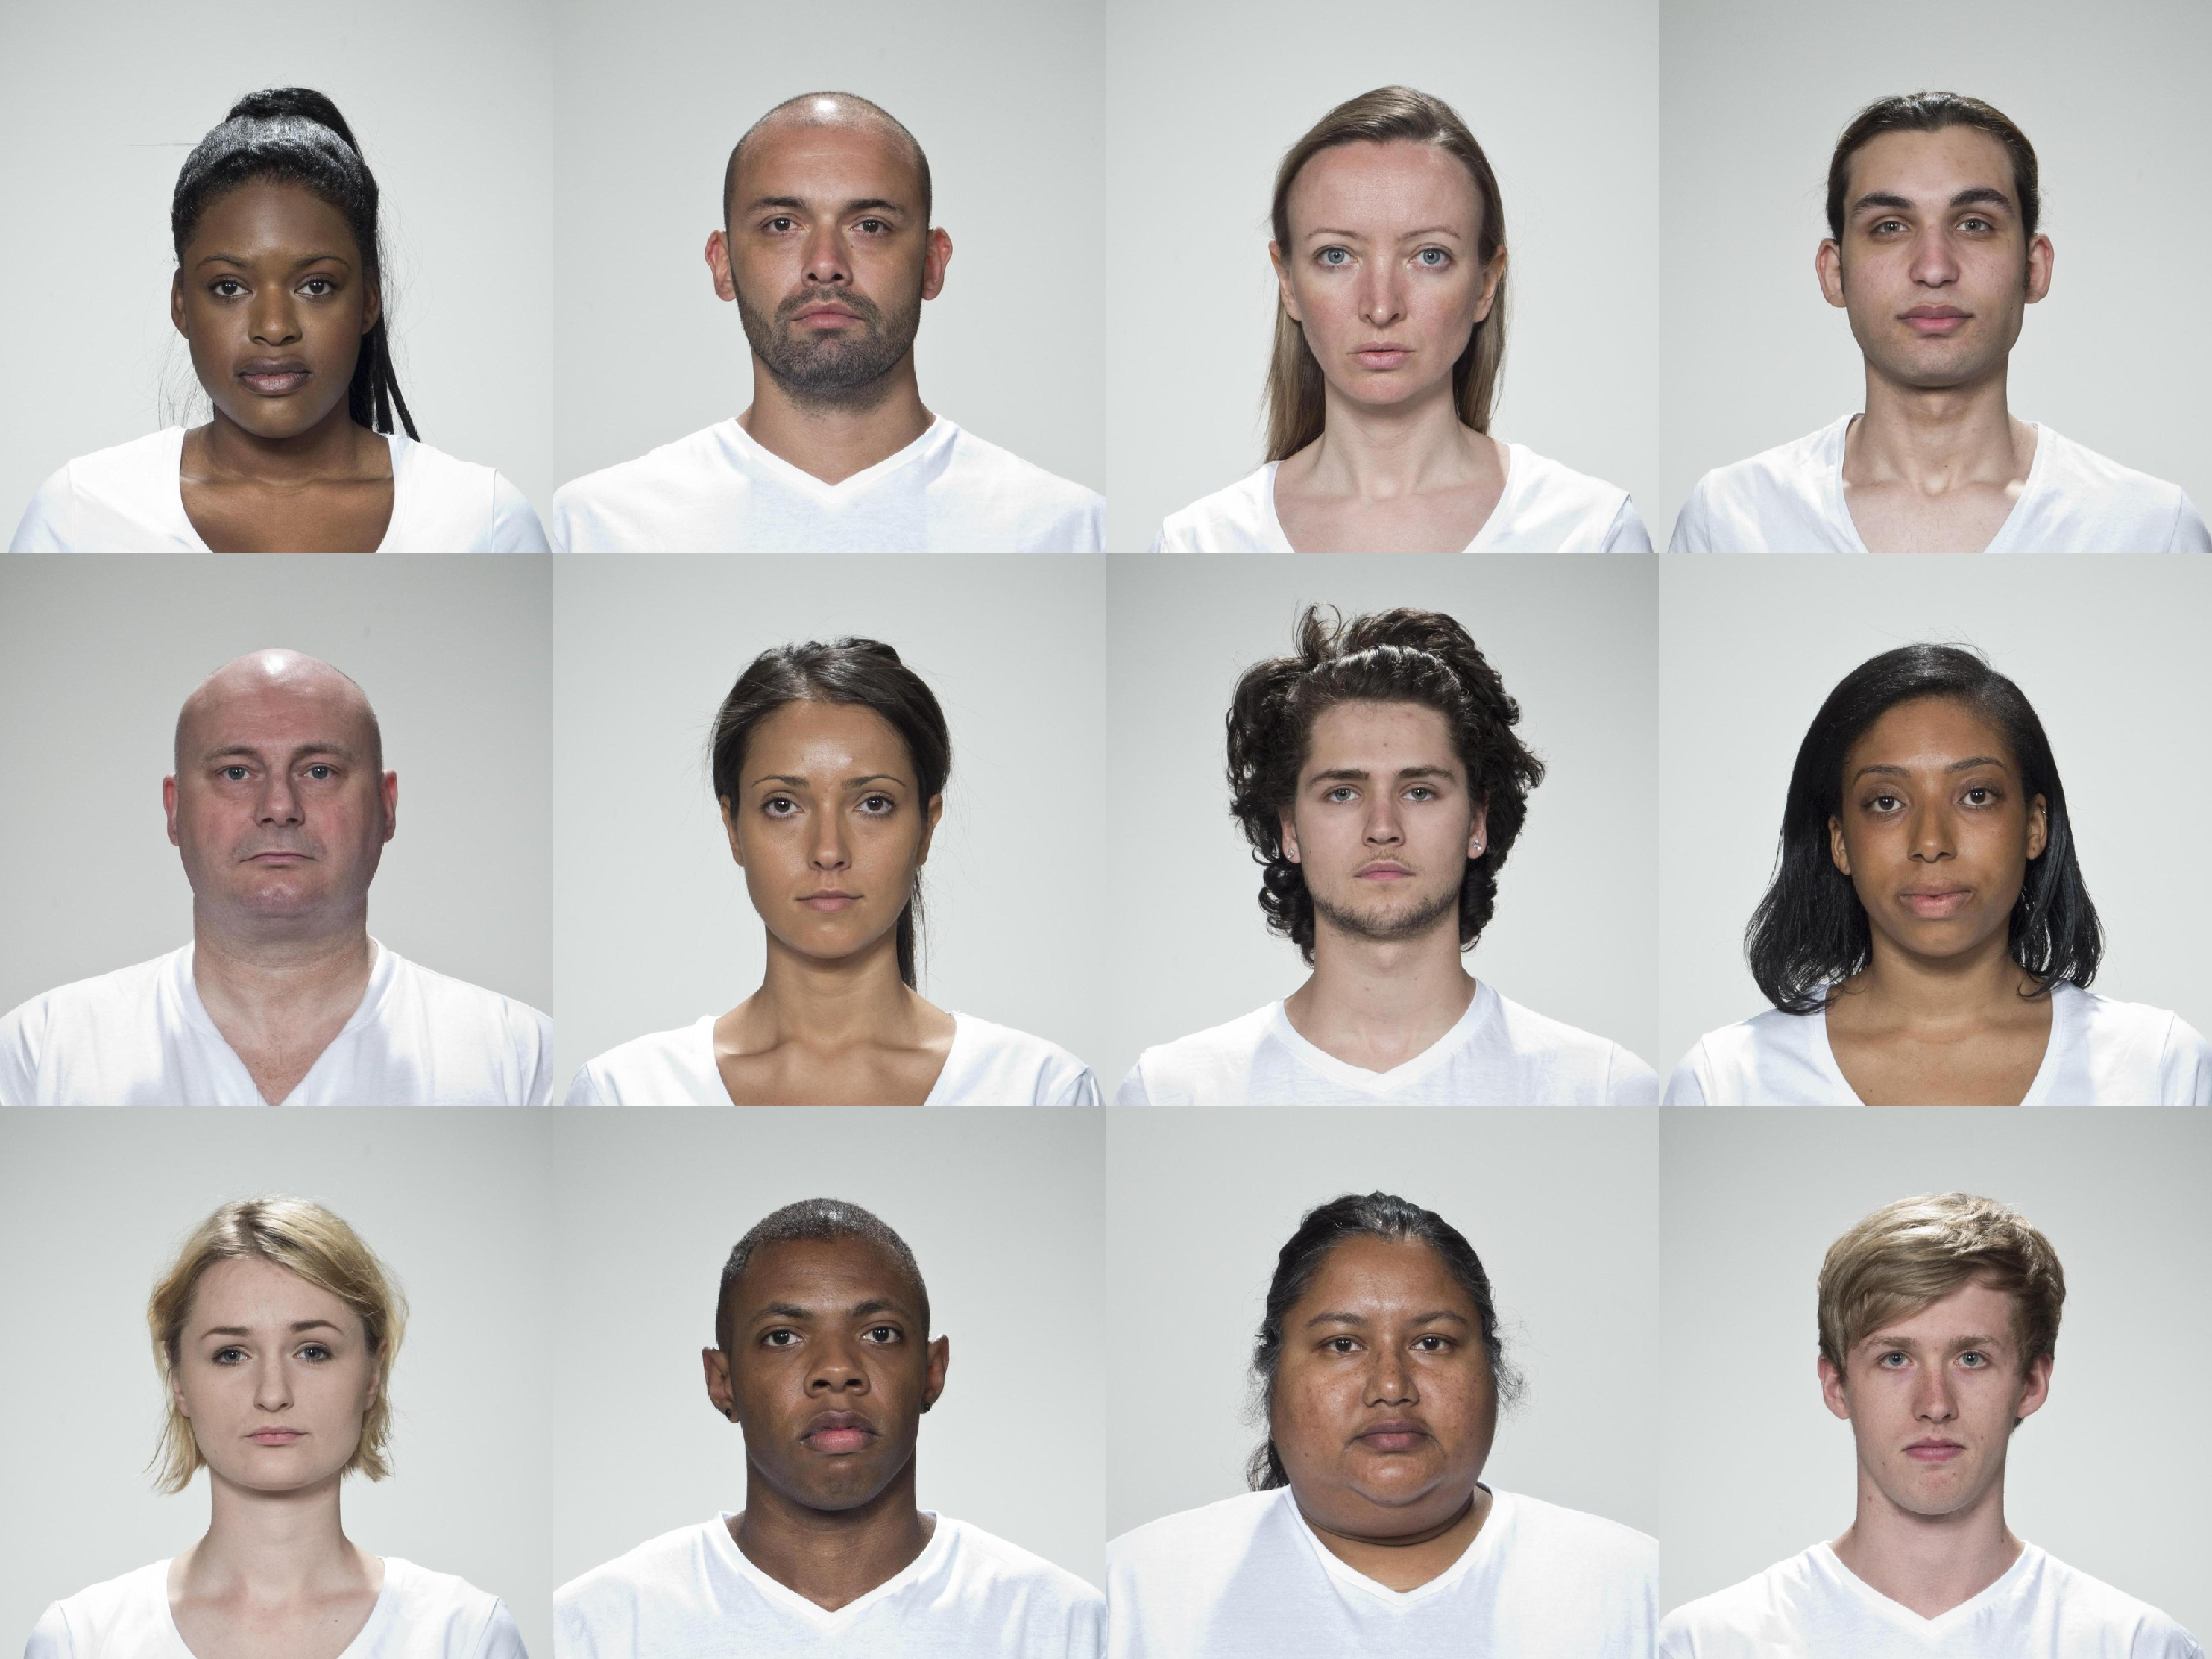
\includegraphics[width=\textwidth]{images/mos_train_set.pdf}\\
        \caption{MOS train set}\label{fig:mos_set_train}
    \end{subfigure}
    \hfill
    \begin{subfigure}{0.19\textwidth}
        \centering
        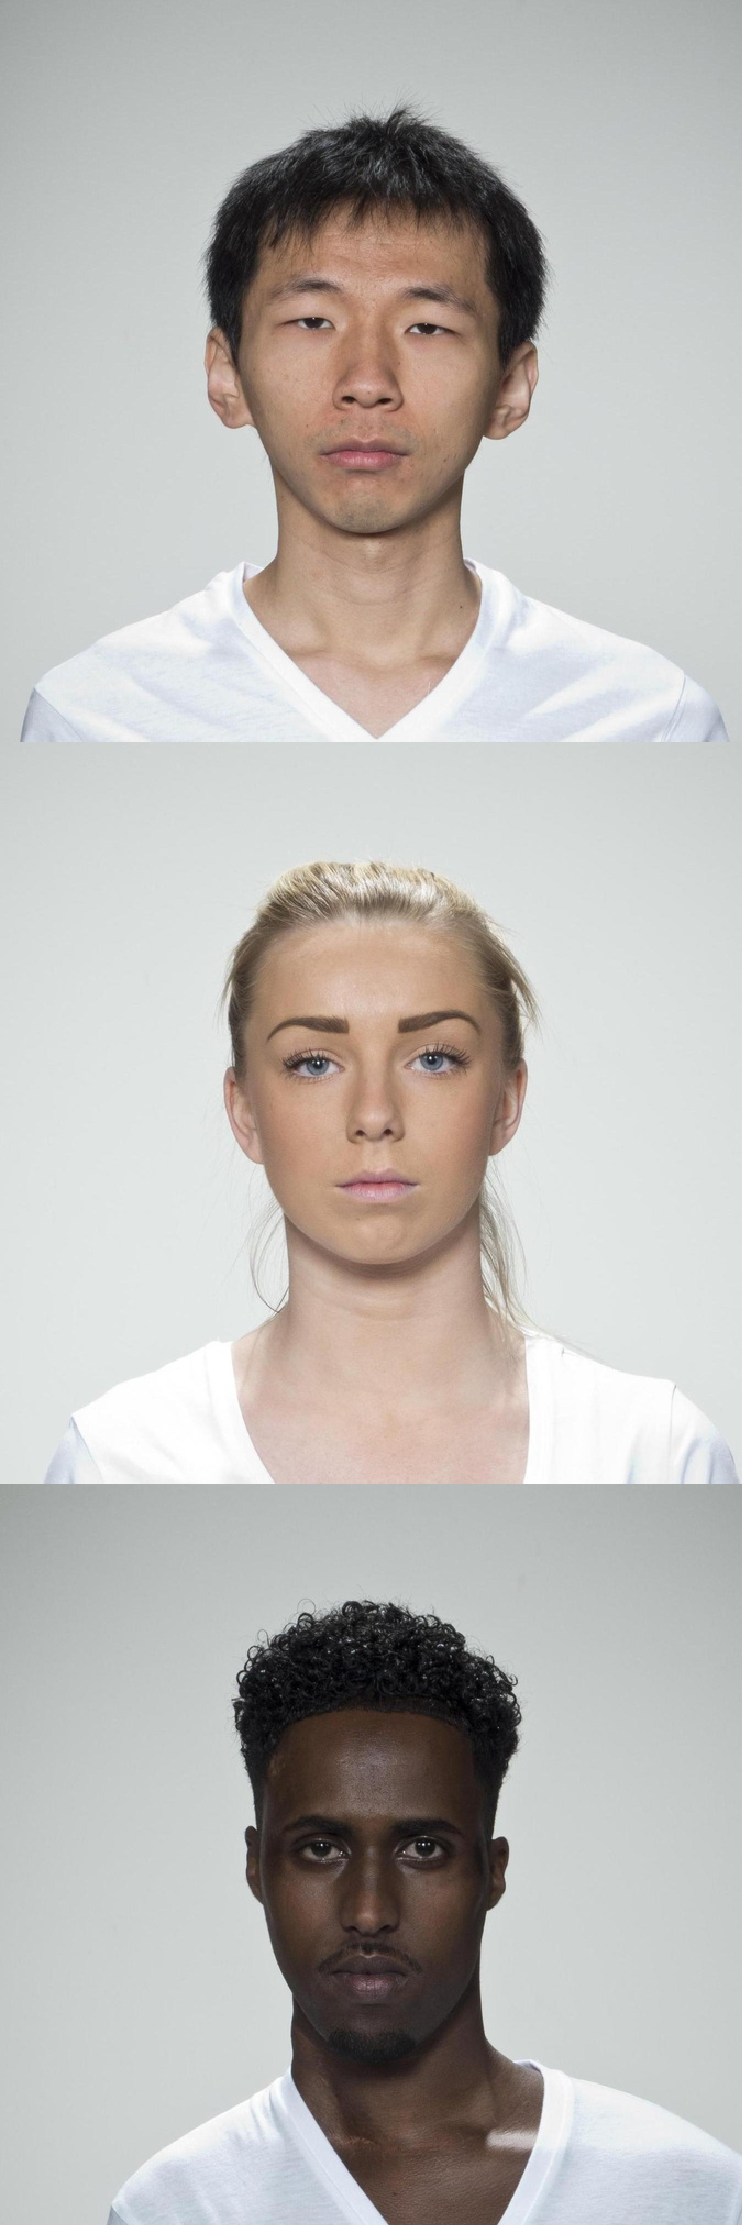
\includegraphics[width=\textwidth]{images/mos_test_set.pdf}\\
        \caption{MOS test set}\label{fig:mos_set_test}
    \end{subfigure}
    \caption{Reference images from the MOS set, comprising the selected subjects from the FRLL dataset.}\label{fig:mos_set}
\end{figure}

The steganographic distortions are visible in Fig.~\ref{fig:steganography}, which shows examples of distorted facial images from each method. The distortions are applied to the original images, and the resulting stego images are used for both subjective evaluation and training of the NR-IQA model. The selected steganographic methods represent diverse classes of distortion processes (geometric, color-based, local texture perturbation) commonly encountered in practical steganographic applications. The chosen intensity levels ensure a broad perceptual range from barely noticeable to clearly visible distortions.

\begin{figure}
    \centering
    \begin{subfigure}{0.23\textwidth}
        \centering
        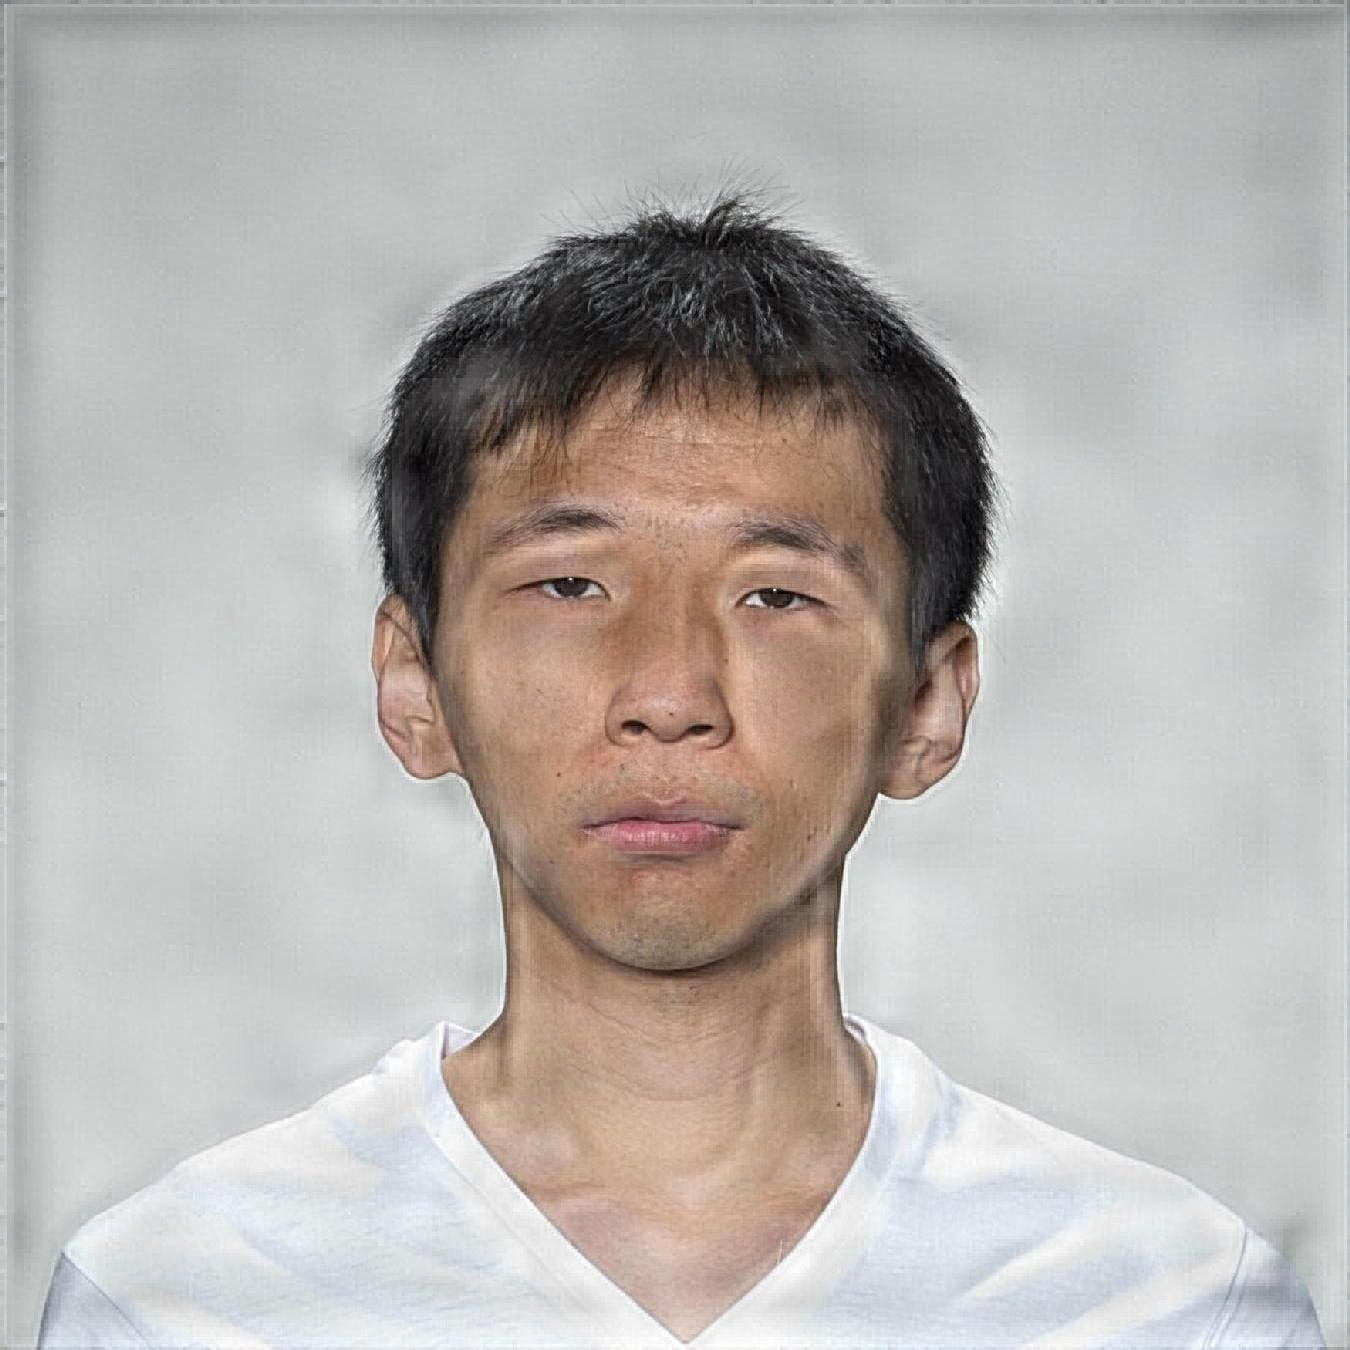
\includegraphics[width=\textwidth]{images/005_StegaStamp_1.4.jpg}\\
        \caption{StegaStamp}\label{fig:steganography_a}
    \end{subfigure}
    \hfill
    \begin{subfigure}{0.23\textwidth}
        \centering
        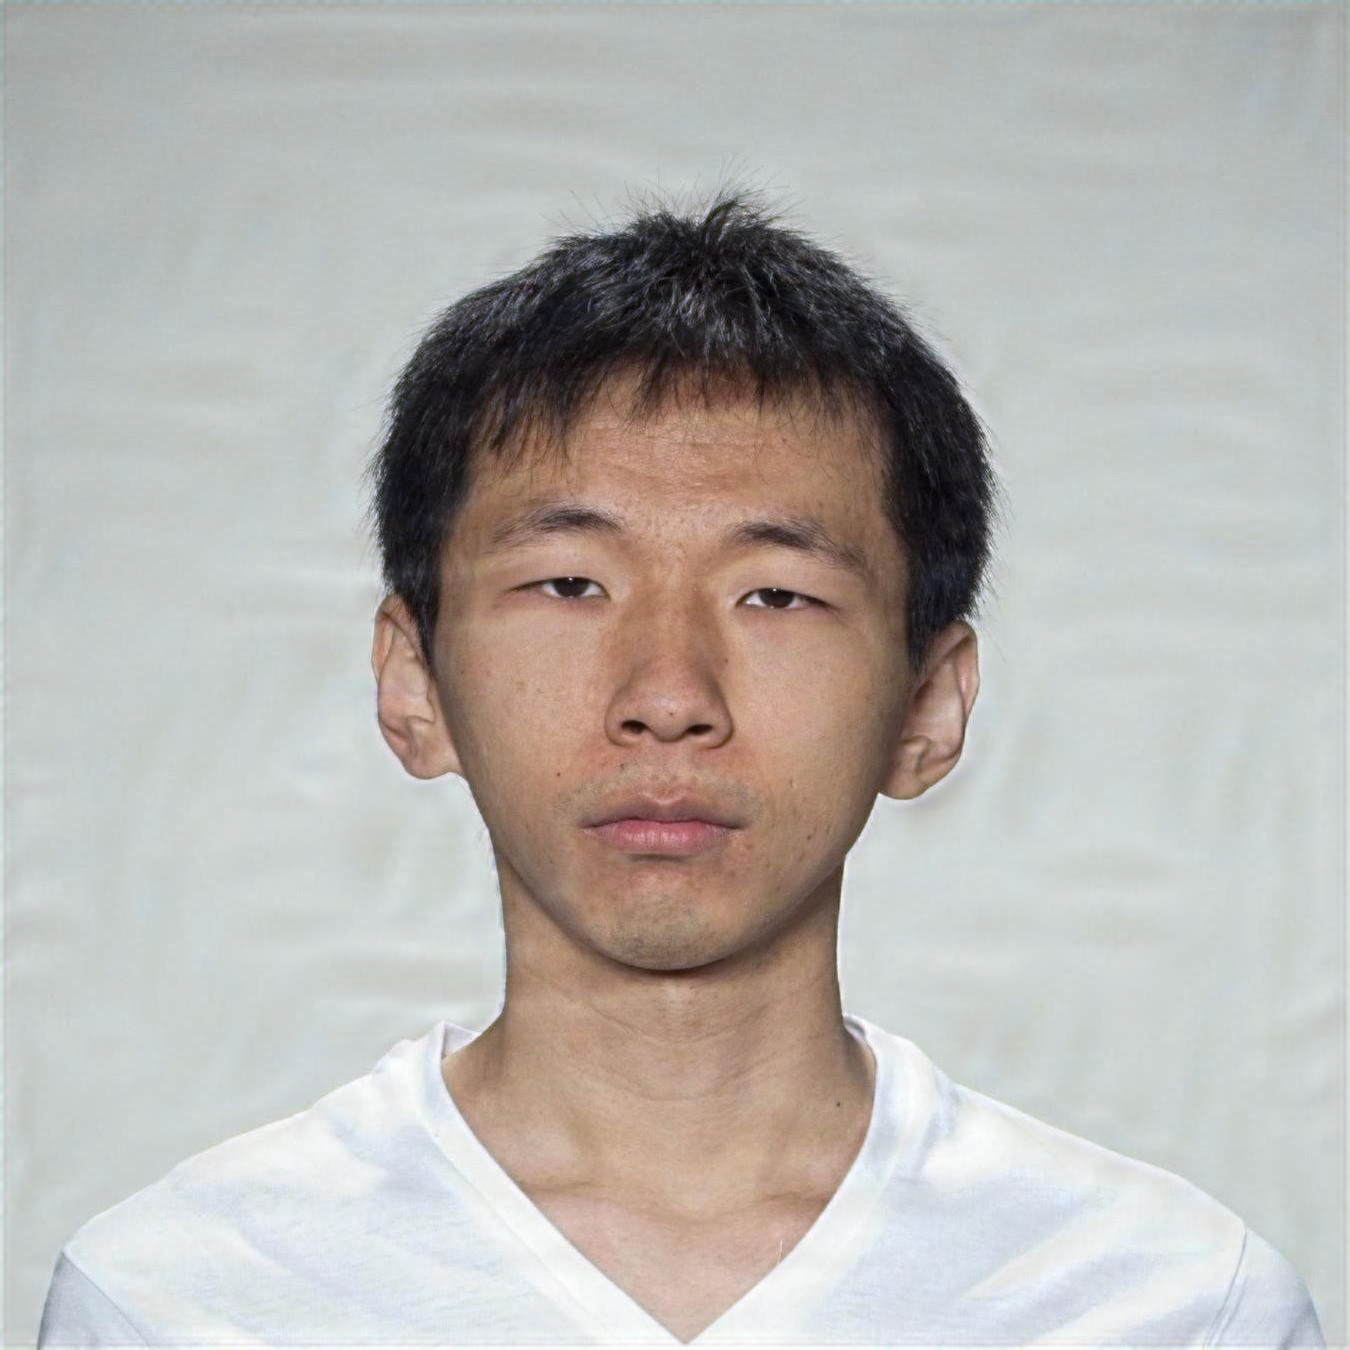
\includegraphics[width=\textwidth]{images/005_CodeFace_1.4.jpg}\\
        \caption{Code\,Face}\label{fig:steganography_b}
    \end{subfigure}
    \hfill
    \begin{subfigure}{0.23\textwidth}
        \centering
        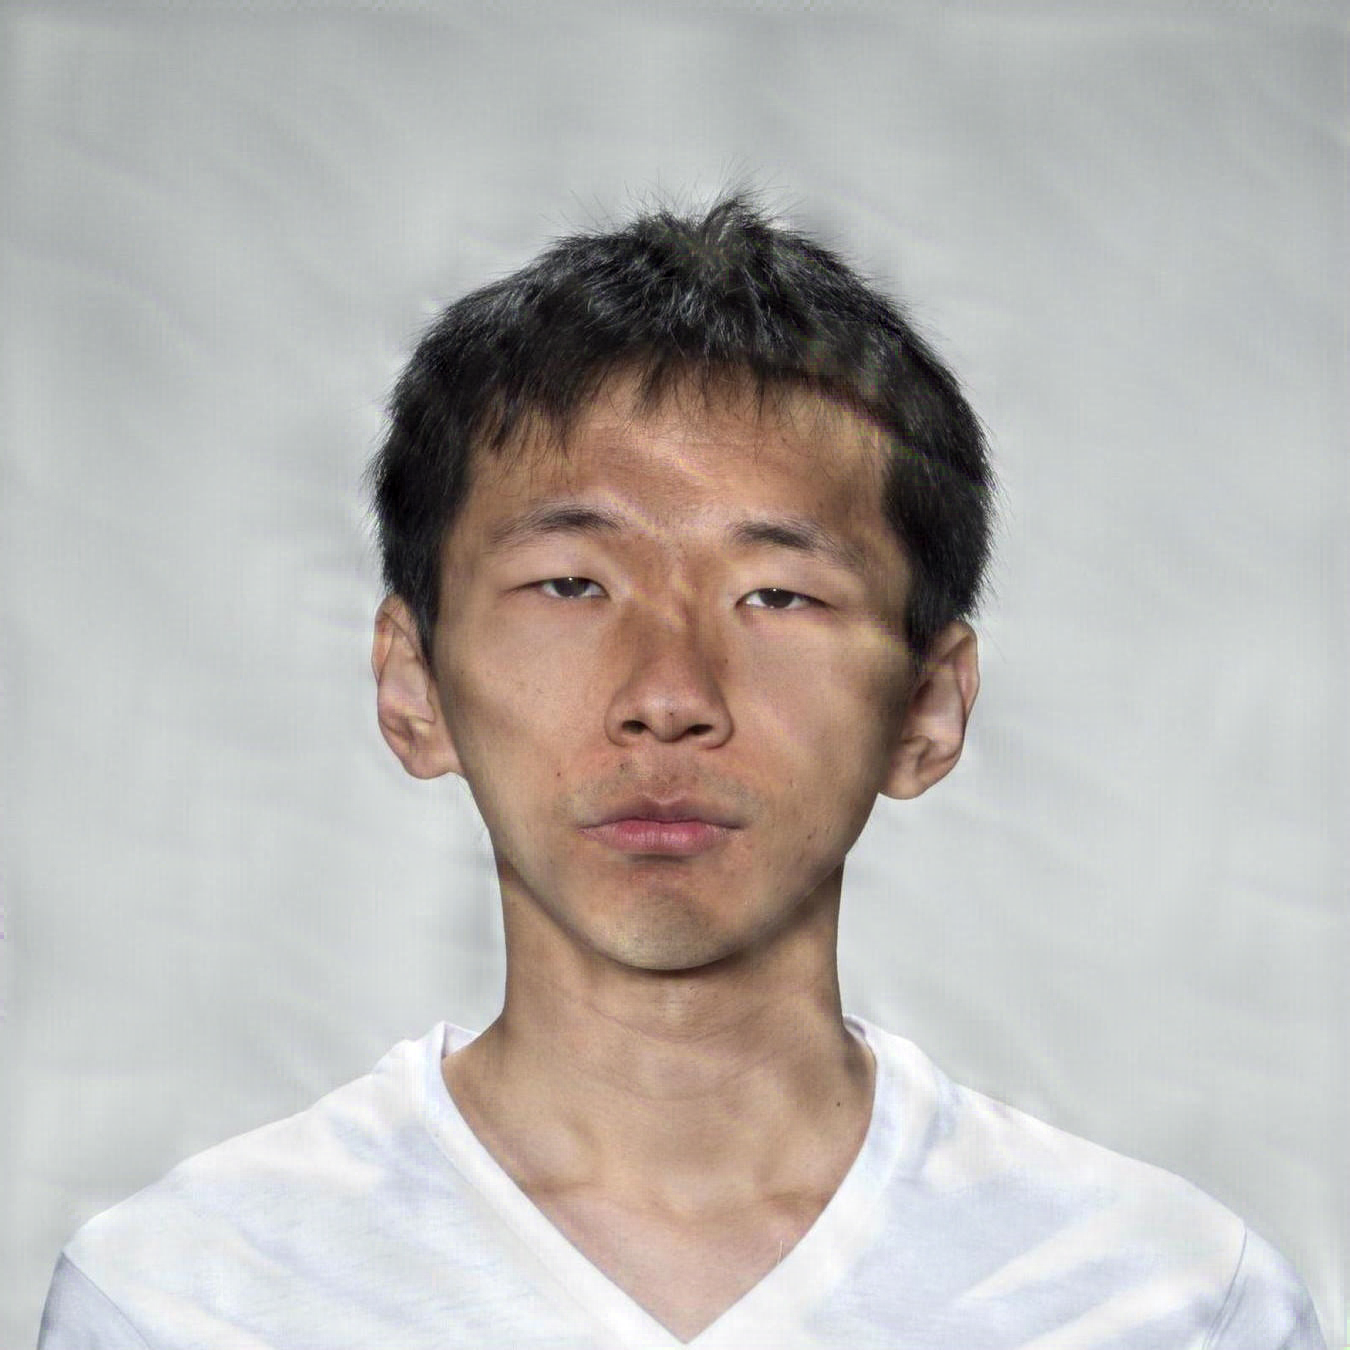
\includegraphics[width=\textwidth]{images/005_RiemStega_1.4.jpg}\\
        \caption{RiemStega}\label{fig:steganography_c}
    \end{subfigure}
    \hfill
    \begin{subfigure}{0.23\textwidth}
        \centering
        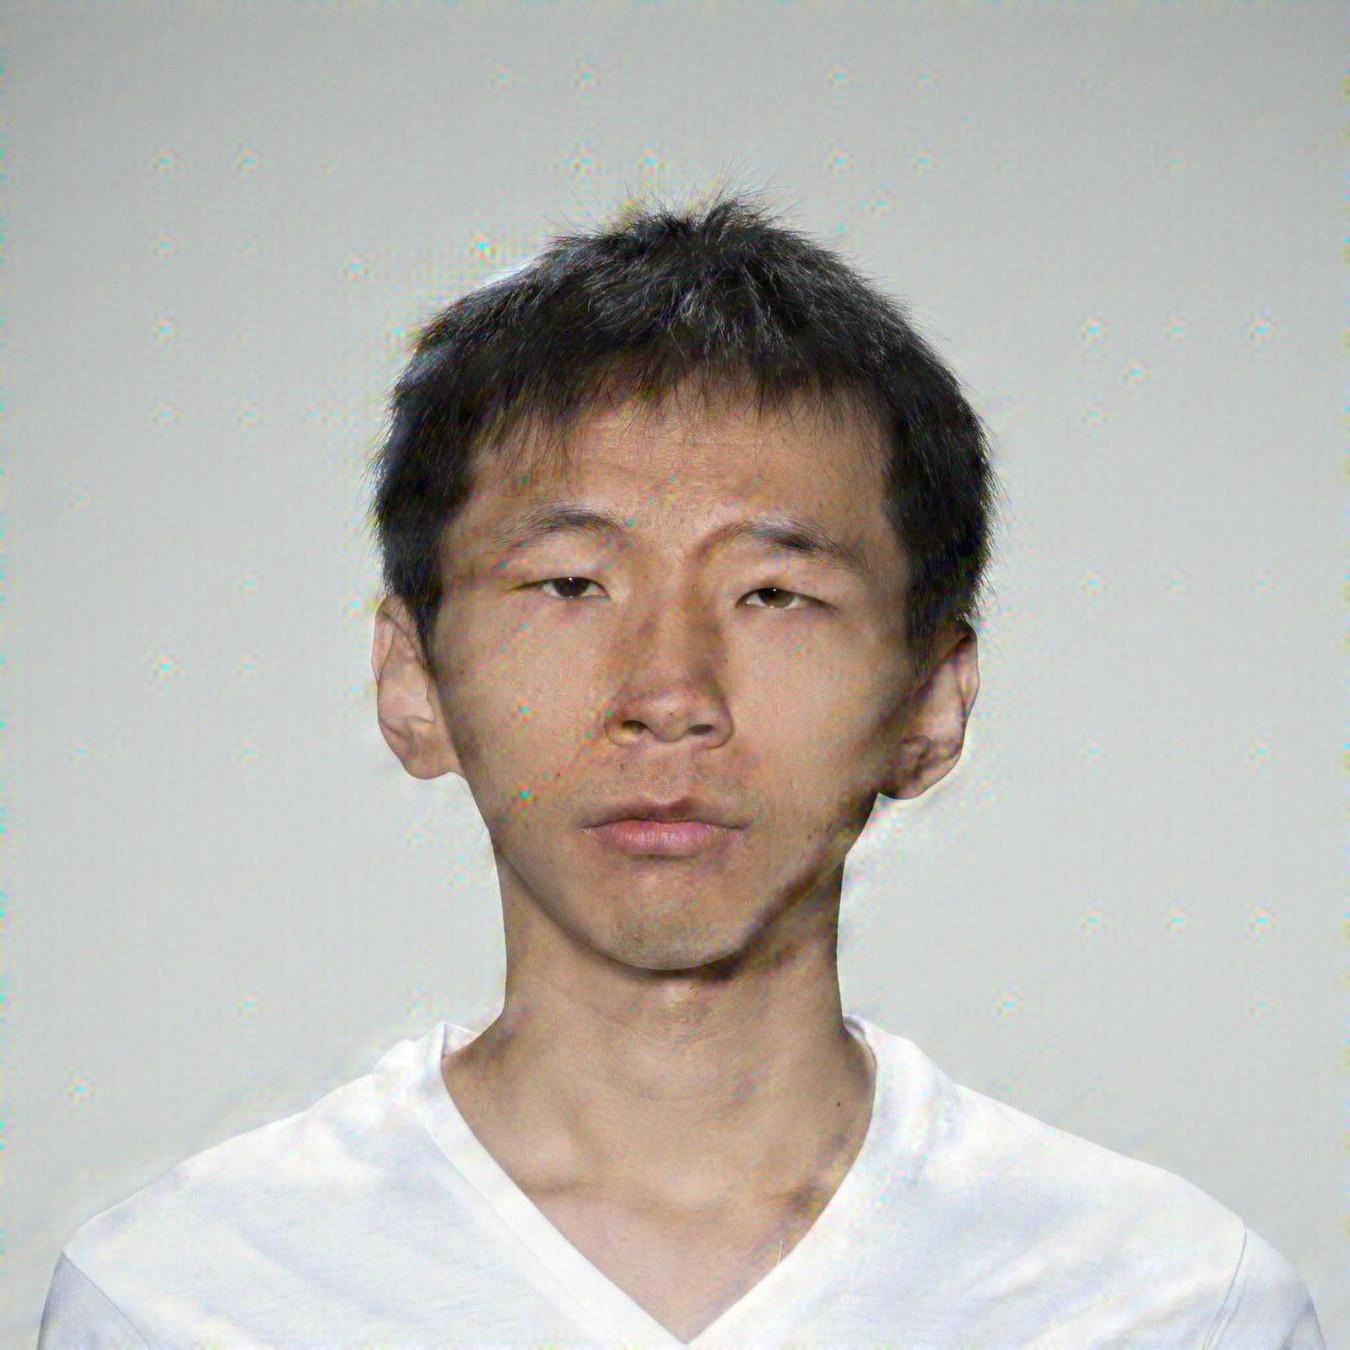
\includegraphics[width=\textwidth]{images/005_StampOne_1.4.jpg}\\
        \caption{StampOne}\label{fig:steganography_d}
    \end{subfigure}
    \caption{Steganographically distorted facial images from each method.}\label{fig:steganography}
\end{figure}

\section{Collection of Subjective Scores}

We followed the ITU-R BT.500--15~\cite{ITU-R-BT500} recommendation and adopted the Single Stimulus (SS) method. The test was implemented using a custom Django web application seen in Fig.~\ref{fig:webapp}. Prior to the test session, participants signed an informed consent form and filled out a registration form providing demographic and environmental information such as age, gender, education, country of origin and ethnicity, and others. Each image was shown individually, with no time limit. Ratings were submitted using a labeled slider, and automatic saving ensured session robustness.

\begin{figure}
    \centering
    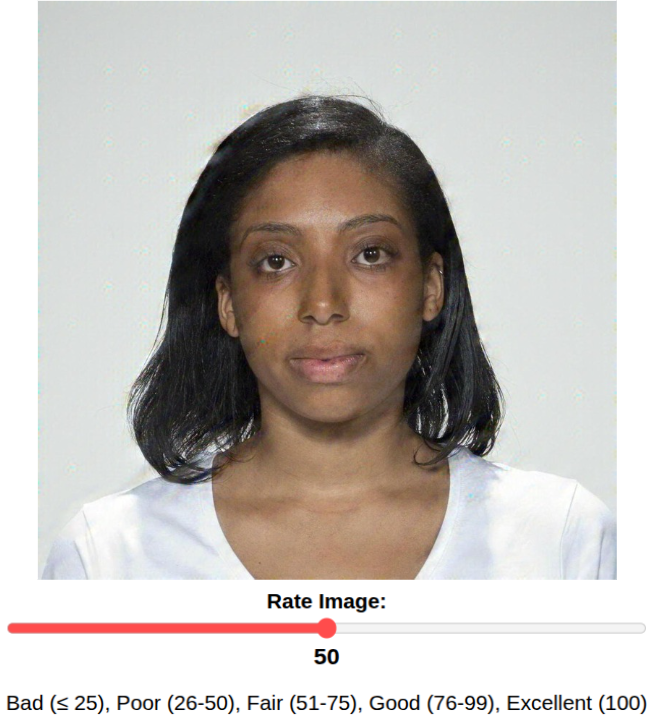
\includegraphics[width=0.5\textwidth]{images/webapp_test.png}
    \caption{Django-based webapp created for the Single Stimulus test.}\label{fig:webapp}
\end{figure}

Each image in the MOS set was evaluated approximately 30 times by human observers, resulting in over 14,000 ratings. We had around 200 participants, each session lasted about 22 minutes and included roughly 70 evaluations. Table~\ref{tab:demographics} summarizes the demographic profile of the participant pool. Following the session, outlier observers were identified and removed using both Kurtosis-based and correlation-based post-screening methods described in ITU-R BT.500--15~\cite{ITU-R-BT500}, resulting in the exclusion of one participant.

\begin{table}
    \centering
    \caption{Demographic and non-demographic profile of the observers.}
    \label{tab:demographics}

    % First row of subtables
    \begin{subtable}{0.3\textwidth}
        \centering
        \caption{Age group}
        \begin{tabular}{lr}
            \hline
            Group & Count \\
            \hline
            18--25 & 85 \\
            26--40 & 54 \\
            41--60 & 52 \\
            Above 60 & 9 \\
            Under 18 & 2 \\
            \hline
        \end{tabular}
    \end{subtable}
    \hfill
    \begin{subtable}{0.3\textwidth}
        \centering
        \caption{Gender}
        \begin{tabular}{lr}
            \hline
            Gender & Count \\
            \hline
            Male & 143 \\
            Female & 59 \\
            \hline
        \end{tabular}
    \end{subtable}
    \hfill
    \begin{subtable}{0.3\textwidth}
        \centering
        \caption{Ethnicity}
        \begin{tabular}{lr}
            \hline
            Group & Count \\
            \hline
            White & 177 \\
            Latino & 8 \\
            Black & 6 \\
            Mixed / Multiple & 3 \\
            Others & 7 \\
            \hline
        \end{tabular}
    \end{subtable}

    \vfill

    \begin{subtable}{0.3\textwidth}
        \centering
        \caption{Education}
        \begin{tabular}{lr}
            \hline
            Level & Count \\
            \hline
            Bachelor's & 92 \\
            Master's & 63 \\
            Doctorate & 29 \\
            High School & 14 \\
            Other & 4 \\
            \hline
        \end{tabular}
    \end{subtable}
    \hfill
    \begin{subtable}{0.3\textwidth}
        \centering
        \caption{Country}
        \begin{tabular}{lr}
            \hline
            Country & Count \\
            \hline
            Portugal & 170 \\
            Brazil & 16 \\
            Russia & 3  \\
            India & 2 \\
            Ghana & 2 \\
            Others & 9 \\
            \hline
        \end{tabular}
    \end{subtable}
    \hfill
    \begin{subtable}{0.3\textwidth}
        \centering
        \caption{Device Used}
        \begin{tabular}{lr}
            \hline
            Device & Count \\
            \hline
            Laptop & 94 \\
            Phone & 65 \\
            Desktop & 42 \\
            Other & 1 \\
            \hline
        \end{tabular}
    \end{subtable}
\end{table}



The database was implemented using the Django web framework, which provides an object-relational mapping (ORM) layer that directly maps Python model classes to database tables. The ORM also enforces data integrity constraints and simplifies querying for statistical analysis. The database backend used was PostgreSQL.

The database schema was designed to ensure structured storage and traceability of all subjective quality evaluation data. Fig.~\ref{fig:db_conceptual} presents the conceptual data model, which defines the main entities and their relationships. The profile entity stores participant metadata, including age, gender, education, ethnicity, country of origin, and device used. The ss\_session entity models individual test sessions and is linked to both the participant profile and the dataset being evaluated. The image entity encodes each image's filename, associated distortion type (distortion\_name), and distortion level (distortion\_level). The test entity stores individual subjective ratings, including the precise timestamp of submission, linked to both the session and the image presented. An auxiliary user\_feedback entity captures optional, anonymous, observer comments and critiques.

The physical implementation of this schema, shown in Fig.~\ref{fig:db_physical}, is realized as a relational database with explicit foreign key constraints to ensure referential integrity. The dataset\_id and profile\_id fields in ss\_session formally enforce the linkage to specific datasets and participants. The test table connects each subjective rating to its session (ss\_session\_id) and image (image\_id), enabling consistent aggregation of ratings into a statistical descriptors such as MOS and confidence intervals per image and per distortion level. The relational model also facilitates efficient querying for downstream statistical analysis and supports reproducibility of the experimental protocol in line with ITU-R BT.500-15 recommendations.

\begin{figure}
    \centering
    \begin{subfigure}{0.8\textwidth}
        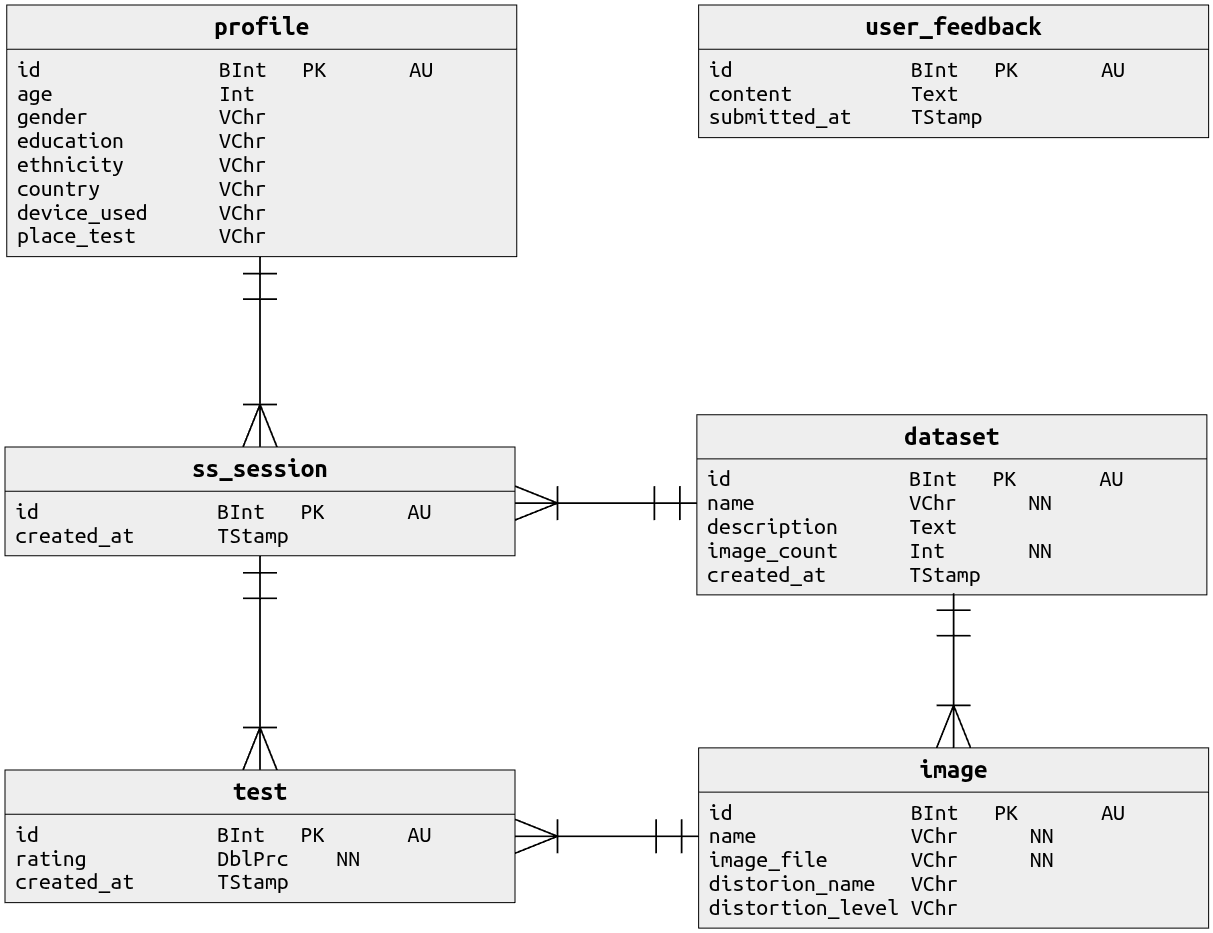
\includegraphics[width=\textwidth]{images/db_conceptual.png}
        \caption{Conceptual database schema showing entity relationships and high-level structure.}\label{fig:db_conceptual}
    \end{subfigure}
    \vfill
    \begin{subfigure}{0.8\textwidth}
        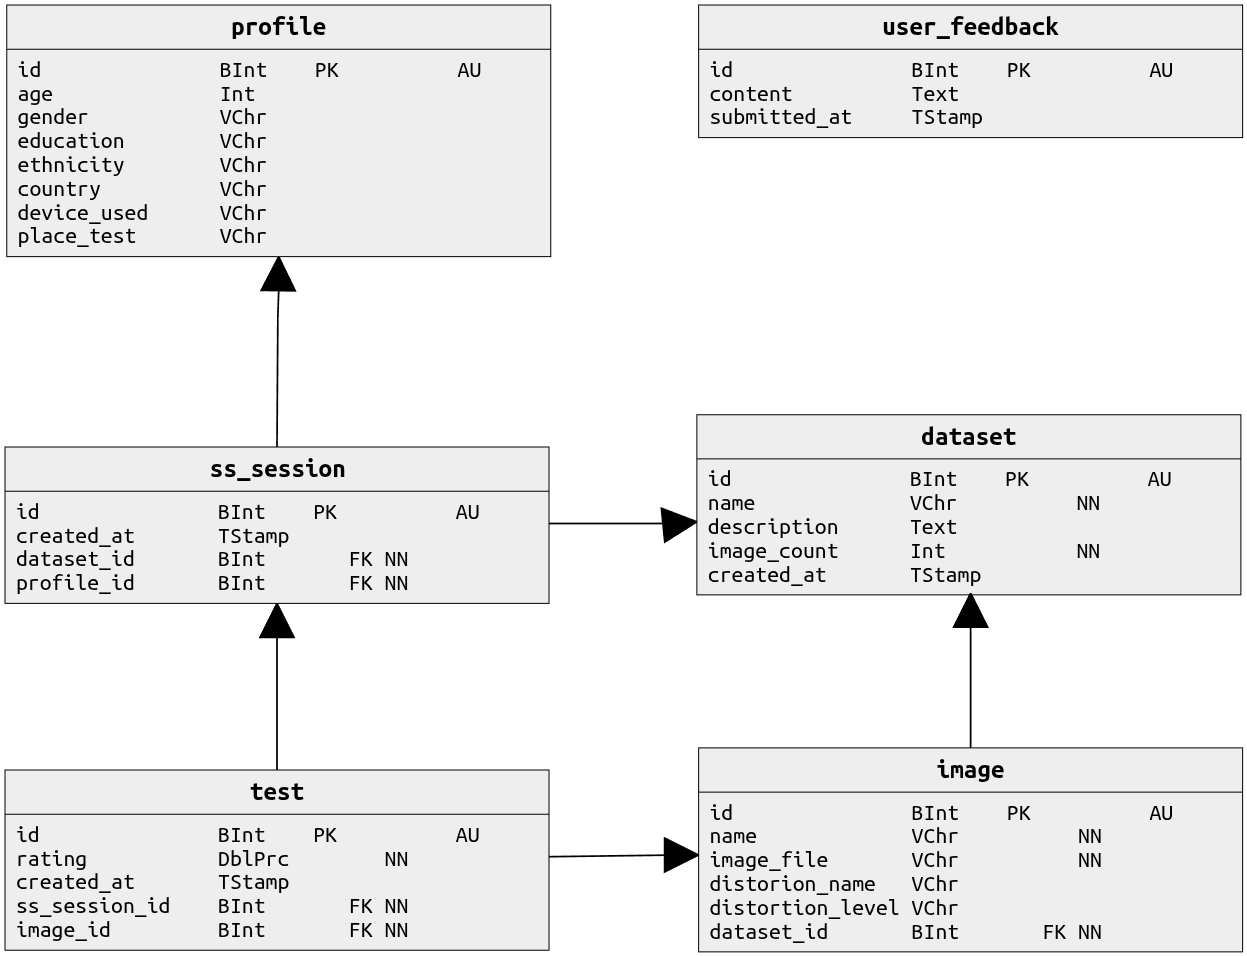
\includegraphics[width=\textwidth]{images/db_physical.png}
        \caption{Physical database schema illustrating actual tables, columns, and implementation details.}\label{fig:db_physical}
    \end{subfigure}
    \caption{Conceptual and physical representations of the database schema.}\label{fig:db_schemas}
\end{figure}


\section{Debiasing of Subjective Scores}

To correct for demographic bias in the subjective scores, we followed a procedure inspired by prior work on bias correction in perceptual tasks~\cite{clapes2018apparent}, where we applied a residualization method based on linear modeling. An ordinary least squares (OLS) regression was fit to the MOS values, using observer and image attributes, and their pairwise interactions as categorical predictors. The fitted bias components were subtracted from the original scores, and the residuals were mean-centered to preserve the global score distribution. As shown in Table~\ref{tab:anova}, several factors exhibit statistically significant effects on the MOS prior to residualization, notably observer and subject ethnicity. After applying the residualization procedure, these effects disappear, as confirmed by an ANOVA test showing no significant impact from any individual factor. The corrected MOS labels are then used as ground truth in all supervised stages of the pipeline to ensure fairness and reduce the influence of socially conditioned priors.

\begin{table}
    \centering
    \caption{ANOVA~\cite{ross2017one} results for observer and image attributes. Before debiasing, several factors show statistically significant effects on MOS, p-value $< 0.05$.\@ After residualization, all main effects show no significant impact, confirming the effectiveness of the debiasing procedure.}\label{tab:anova}
    \begin{tabular}{lcc}
        \hline % chktex 44
        Factor & p-value & p-value (residualized) \\
        \hline % chktex 44
        Observer gender                             & 0.022                 & 0.9930 \\
        Observer ethnicity                          & $8.44 \times 10^{-4}$ & 1 \\
        Subject gender                              & $1.60 \times 10^{-3}$ & 0.9722 \\
        Subject ethnicity                           & $7.36 \times 10^{-3}$ & 1 \\
        Observer gender $\times$ Subject gender     & 0.6417              & 0.6417 \\
        Observer ethnicity $\times$ Subject ethnicity & 0.0582              & 0.0582 \\
        \hline % chktex 44
    \end{tabular}
\end{table}

\section{Correlation of FR-IQA Metrics with Human Perception}

We compute 40 FR-IQA scores for each distorted image in the dataset and compare them against the corresponding MOS, as seen in Fig.~\ref{fig:mos_vs_iqa}. Several metrics exhibit strong linear trends with MOS, while others are poorly aligned or even negatively correlated. For a detailed description of these metrics, we refer the reader to~\cite{shahrukh2019survey}.



\begin{figure}
    \centering
    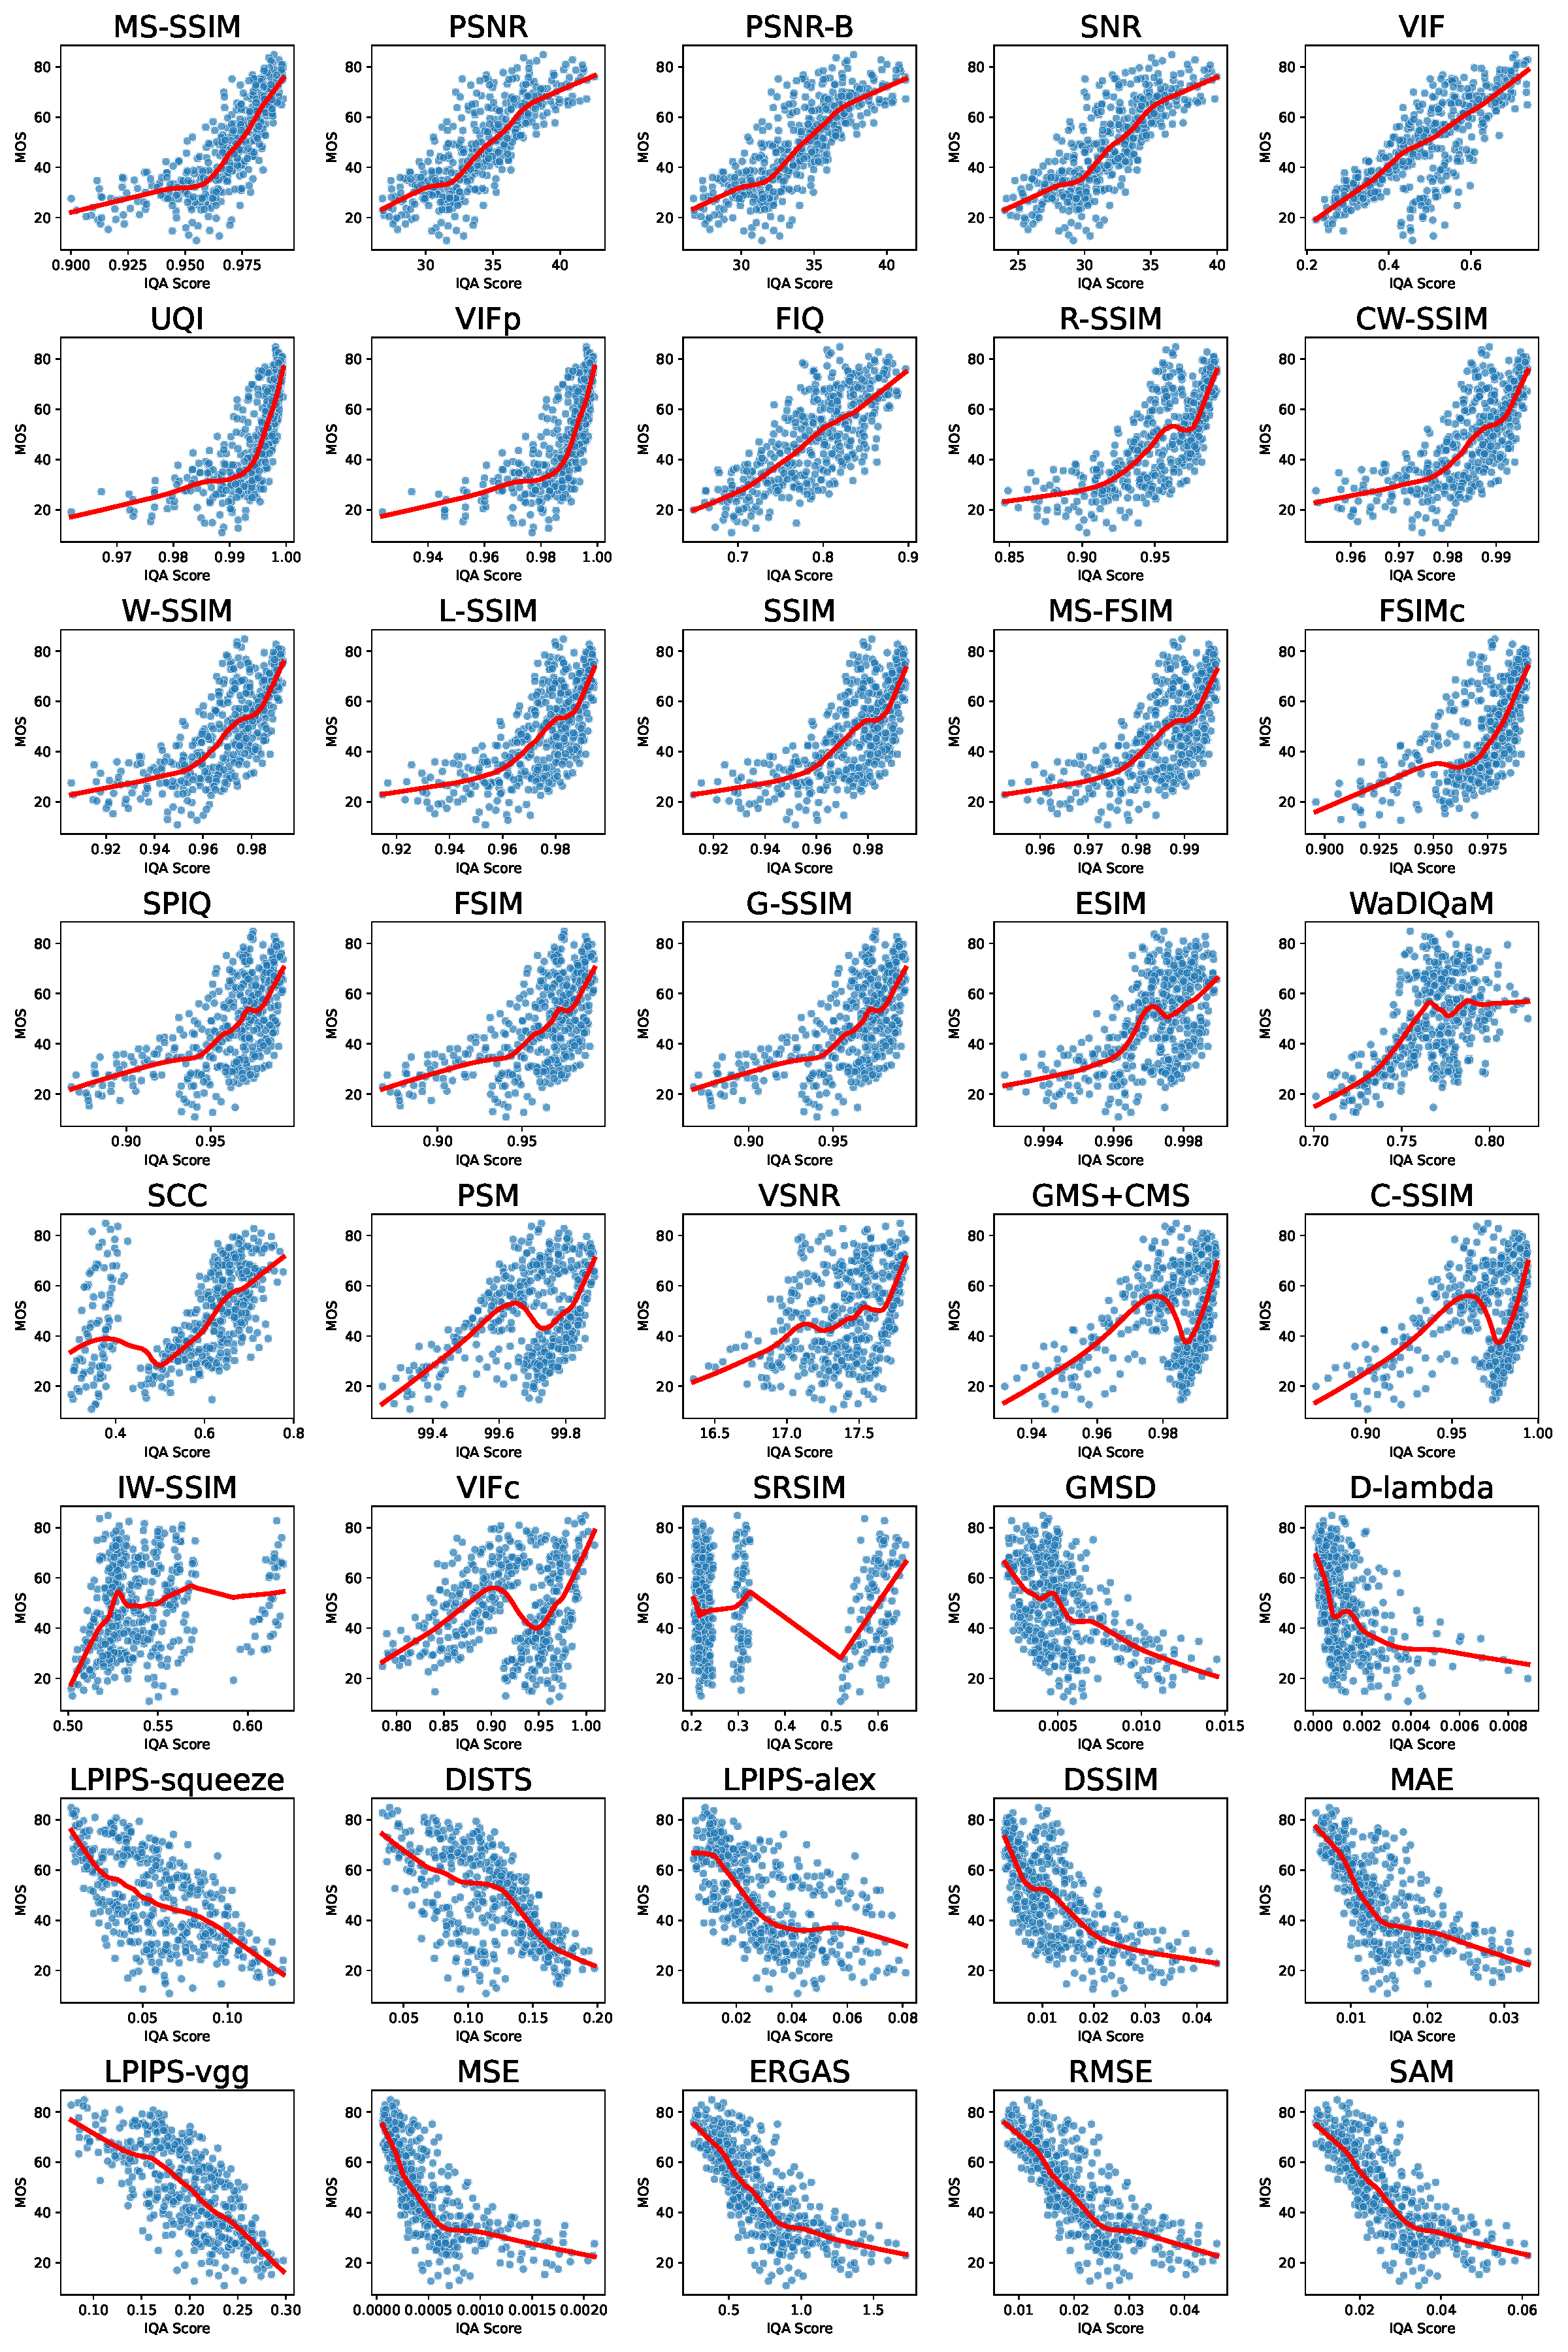
\includegraphics[width=0.90\linewidth]{images/mos_vs_iqa_grid.pdf}
    \caption{Scatter plots illustrating the relationship between MOS and 40 individual full-reference IQA metrics. The red line represents a smoothed local trend curve.}\label{fig:mos_vs_iqa}
\end{figure}

\section{Fusion of FR-IQA Metrics for Pseudo-MOS Estimation}

To identify which metrics align best with human perception, we compute both the Pearson Linear Correlation Coefficient (PLCC) and the Spearman Rank-Order Correlation Coefficient (SRCC)~\cite{plcc-srcc} which respectively quantify the linearity and monotonicity of the relationship between metric scores and MOS.\@ To determine the appropriate number of metrics to retain for fusion, we applied Singular Value Decomposition (SVD) and the Picard criterion~\cite{hansen1998picard}. Metrics are first ranked by the average of their PLCC and SRCC with MOS.\@ After normalizing the feature matrix, SVD revealed that six components capture 95\% of the total variance, as shown in Fig.~\ref{fig:svd_analysis}a, indicating an optimal dimensionality of $k=6$.

To validate this truncation point, we examined the Picard plot in Fig.~\ref{fig:svd_analysis}b, which compares singular values with the target projections. The stable ratio in the tail confirms that six components provide a good balance between expressiveness and stability. This supports a compact, informative subset of FR-IQA metrics.

\begin{figure}
    \centering
    \begin{minipage}{0.48\textwidth}
        \centering
        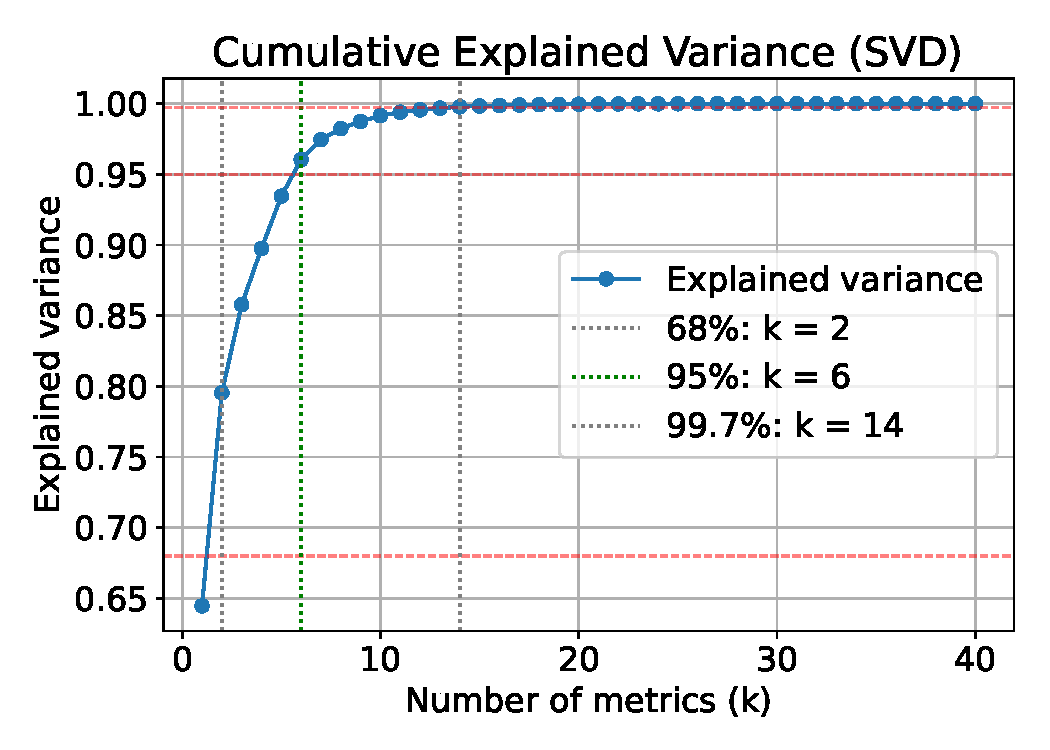
\includegraphics[width=\linewidth]{images/variance.pdf}
        \textbf{(a)} Cumulative variance explained by SVD components.
    \end{minipage}
    \hfill
    \begin{minipage}{0.48\textwidth}
        \centering
        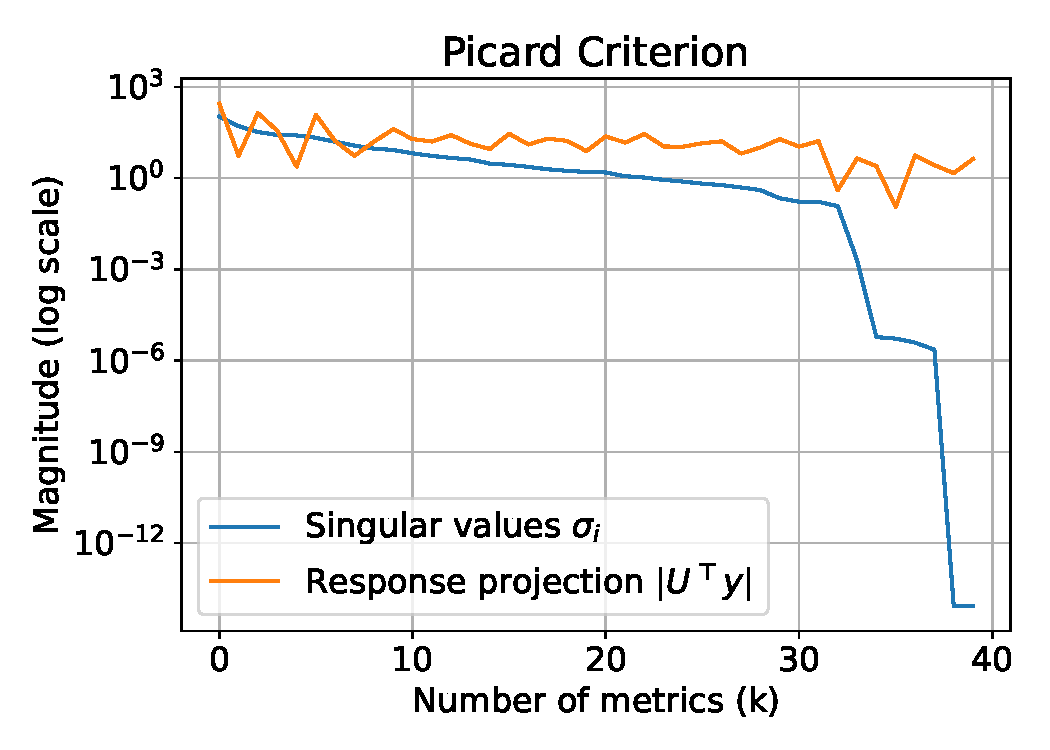
\includegraphics[width=\linewidth]{images/picard.pdf}
        \textbf{(b)} Magnitude of singular values and projected response.
    \end{minipage}
    \caption{SVD-based analysis of the FR metric space. The cumulative explained variance (a) guides the choice of dimensionality, while the Picard criterion (b) illustrates stability near $k=6$.}\label{fig:svd_analysis}
\end{figure}

After selecting the top $k = 6$ FR-IQA metrics, we trained a diverse set of supervised regressors to map these features to subjective MOS scores. The models included both linear and non-linear types:

\begin{itemize}
    \item Linear models: Linear Regression~\cite{linearregression}, Ridge Regression~\cite{ridgeregression}, Bayesian Ridge~\cite{bayesianridge}, ElasticNet~\cite{elasticnet}.
    \item Kernel-based: Support Vector Regression~\cite{svr} (SVR).
    \item Ensembles: Random Forest~\cite{randomforest}, Extra Trees~\cite{ensembles}, Gradient Boosting~\cite{gradboosting}, HistGradientBoosting~\cite{histboost}.
    \item Boosted Trees: XGBoost\cite{xgboost}, LightGBM~\cite{lightgbm}, CatBoost~\cite{catboost}.
\end{itemize}

Each regressor was trained using five-fold cross-validation with an exhaustive grid search over predefined hyperparameter spaces. The best model, CatBoost, optimal configuration was: depth = 8, iterations = 500, learning rate = 0.05, and $L_2$ regularization = 1. This trained regressor is then applied to the unlabeled portion of the dataset (3,132 distorted images), generating pseudo-MOS.\@

\section{Training a No-Reference IQA Model from Pseudo-MOS}

To enable NR quality prediction, we train a deep regression model end-to-end using pseudo-MOS scores as targets. The architecture is based on a ResNet-18 backbone~\cite{resnet} pretrained on ImageNet~\cite{imagenet}, with its final classification layer replaced by a lightweight multi-layer perceptron (MLP) regressor~\cite{bayesianridge}. All layers are fine-tuned during training to learn perceptual quality representations specific to our task. The training set consists of distorted facial images paired with either pseudo-MOS, from the FR fusion, or real MOS labels, when available. The model is optimized using MSE and evaluated on the, disjoint, MOS test set of labeled images. Once trained, the model infers image quality solely from the distorted input, enabling NR assessment aligned with human perception.

